\setbeamertemplate{footline}[first]

\begin{frame}[noframenumbering]
    \titlepage
    \begin{textblock}{10}(4.75,15)
        \cite{logo}
    \end{textblock}
\end{frame}

\setbeamertemplate{footline}[presentationbody] 

\begin{frame}{Vorstellung}
    \note<4->{
        Erstes Mal Vorlesung, Background nicht in mobilen Applikationen\\Bitte um Geduld, Hinweise\\
        Whiteboard:
        \begin{itemize}
            \item Wer nicht aufgerufen werden will, nach der VL bei mir melden (stelle keine Fragen) oder X oben links bei Antwort
            \item Strichliste: Nur für mich für Gleichmäßigkeit, nicht zensurrelevant
            \item Spontanes, prägnantes, kohärentes Sprechen wichtig! Beispiel: Empfehlung an Politikerin
        \end{itemize}
    }
    \begin{itemize}
        \item<2-> Kurz zu mir
        \only<2-4>{
            \begin{itemize}
                \item<2-4> Kontakt: Piotr.Dabrowski@htw-berlin.de - gerne nutzen!
                \item<2-4> Repository: https://github.com/dabrowskiw/
                \item<3-4> Geboren 1981 in Warschau
                \item<3-4> Studium der Biotechnologie \& Informatik an der TU Berlin
                \item<3-4> Promotion über Auswertung von Hochdurchsatzdaten für Virus-Diagnostik
                \item<3-4> Aufbau der bioinformatischen Analytik für das NGS-Labor des RKI
                \item<3-4> Aufbau der Bioinformatics Core Facility am RKI
                \item<3-4> Leitung des Aufgabenbereichs zur Modernisierung der Haushaltsvollzugs-Software des Bundes
                \item<4> Hang zu unkonventionellen Vorlesungsmethoden - Feedback erwünscht!
            \end{itemize}
        }
        \item<5-> Der Todesstern \& (ausgewählte) andere Hilfsmittel
        \item<9-> Sie \& Ihre Vorstellungen, Motivation und Vorkenntnisse
        \only<10->{
            \begin{itemize}
                \item Kommt gleich!
            \end{itemize}
        }
    \end{itemize}
    \only<5-8>{
        \begin{textblock}{15}(2,7)
            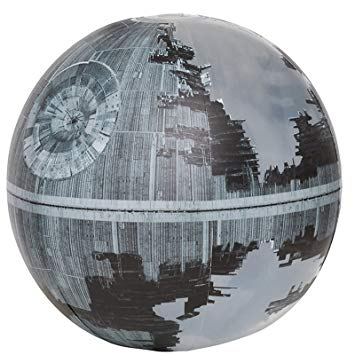
\includegraphics[width=3cm]{Bilder/Todesstern.jpg}
        \end{textblock}
    }
    \only<6-8>{
        \begin{textblock}{15}(5.5,8.25)
            
\includegraphics[width=3cm]{Bilder/Tischnamensschild.png}
        \end{textblock}
    }
    \only<7-8>{
        \begin{textblock}{15}(9,7.5)
            
\includegraphics[angle=77,origin=c,height=2cm]{Bilder/Tischnamensschild.png}
        \end{textblock}
    }
    \only<8>{
        \begin{textblock}{15}(11.5,8)
            
\includegraphics[width=3cm]{Bilder/Whiteboard.png}
        \end{textblock}
    }
\end{frame}

\begin{frame}{Fragen der Vorlesung}
    \note{
        \begin{itemize}
            \item Entwicklung: Besonders wichtig bei Gesundheitswesen: Stabilität, einfache Anwendbarkeit (patient compliance)
            \item Was sind personenbezogene Daten, wann darf man sie verarbeiten - und wann sollte man sie verarbeiten etc.
        \end{itemize}
    }
    \begin{itemize}
        \item Warum sind mobile Applikationen im Gesundheitswesen sinnvoll? Wo werden sie bereits eingesetzt?
        \item<2-> Worauf muss man bei der Entwicklung mobiler Applikationen für das Gesundheitswesen achten?
        \item<3-> Was sind Herausforderungen im Zusammenhang mit der Verarbeitung potentiell sensitiver Daten?
    \end{itemize} 
\end{frame}

\begin{frame}{Inhalt der Übung}
    Entwicklung einer mobilen medizinischen Applikation.
    \begin{itemize}
        \item<2-> Zusammenfinden in 4 möglichst balancierten Teams (5-6 Personen)
        \item<3-> Entwickeln einer Produktidee
        \item<4-> Erstellung von Strategie, Mockups etc.
        \item<5-> Implementation eines Proof of Concept
        \item<6-> Erstellung einer Produktpräsentation (25 Minuten/Gruppe)
    \end{itemize}
    \only<7->{Credit to: Thorsten Knape.}
\end{frame}

\begin{frame}{Benotung}
    \note{
        \begin{itemize}
            \item PoC nicht ``fertig werden'', Idee und Herangehensweise ausschlaggebend.
            \item Produktpräsentation:
            \begin{itemize}
                \item Ideen, Herausforderungen, Umgehen mit Herausforderungen so darstellen, dass sie für die Anderen nachvollziehbar und nützlich sind!
                \item Vorstellung des PoC: Verkaufsevent, warum sind wir besser als alle anderen!
            \end{itemize}
        \end{itemize} 
    }
    \begin{itemize}
        \item<1-> Projektaufgabe: $70\%$
        \only<2>{
            \begin{itemize}
                \item Funktionsfähiger technischer Prototyp: $20\%$
                \item Dokumentation des Codes (Vorhandensein, Übereinstimmung Dokumentation/Code): $10\%$
                \item Projektdokumentation als PDF/Wiki: $10\%$
                \item Konsistenter Code-Stil: $10\%$
                \item Vorhandensein dokumentierter Tests: $10\%$
                \item Kleinteilige Commits: $10\%$
            \end{itemize}
        }
        \item<3-> Präsentation: $30\%$
        \only<4>{
            \begin{itemize}
                \item 25 Minuten/Gruppe + Fragen
                \item \textbf{Für alle verständliche} Vorstellung wichtiger Gedanken, Herausforderungen, Entscheidungen, Lösungsansätze
                \item PoC-Präsentation mit Verkaufscharakter: Warum ist/wird das die beste App auf der Welt?
                \item Emfpehlung: Story erzählen.
            \end{itemize}
        }
        \item<5-> Abgabe Projektaufgabe (git Release mit allen Elementen) und Slides für Präsentation (Mail mit Anhang): 27.01.2020 12:15 (Eingang Mail + Release-Datum)
        \item<6-> Umgesetzte Verbesserungsvorschläge/Fehlerkorrekturen
        \only<7>{
            \begin{itemize}
                \item $2.5\%$ pro Stück
                \item Maximal 2 pro Semester
                \item Wenn als pull request: Doppelte Punktzahl
            \end{itemize}
        }
    \end{itemize}
\end{frame}

\begin{frame}{Vorläufige Zeitplanung}
    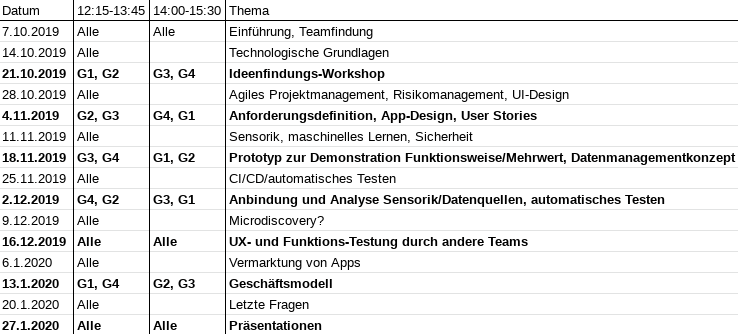
\includegraphics[width=\textwidth]{Bilder/Zeitplan.png}
\end{frame}

\stepcounter{slidesection}
\setbeamertemplate{background}[bgfirst]
\setbeamertemplate{footline}[first]
\subtitle{\theslidesection: Kurzer Einblick in das Gesundheitssystem}
\titlegraphic{Bilder/logo1.png}
\begin{frame}[noframenumbering]
\titlepage
\begin{textblock}{10}(4.75,15)
\cite{GesundheitssystemLogo}
\end{textblock}
\end{frame}
\setbeamertemplate{footline}[presentationbody] 
\setbeamertemplate{background}[bgbody]

\begin{frame}{Begriffsdefinition(en)}
    \begin{definition}
        Das Gesundheitswesen ist die Gesamtheit eines organisierten Handelns als Antwort auf das Auftreten von Krankheit und Behinderung und zur Abwehr gesundheitlicher Gefahren.
    \end{definition}
    \only<2->{
        \begin{definition}
            Das Gesundheitswesen setzt sich aus allen Instituten, Einrichtungen, Personen und allen Maßnahmen zusammen, die für die Bevölkerung gesundheitsfördernd und -erhaltend sind, vorbeugend gegen Verletzungen und Krankheit wirken sowie diese behandeln.
        \end{definition}
    }
\end{frame}

\begin{frame}{Akteure im Gesundheitssystem (Überblick)}
    \begin{figure}[h!]
        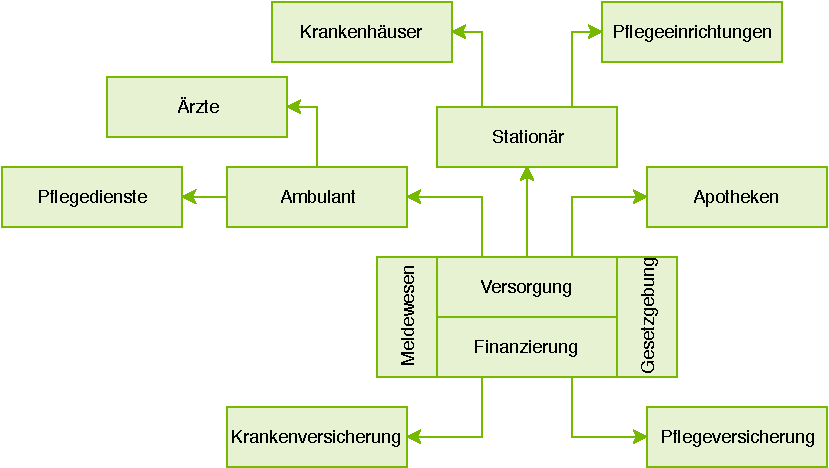
\includegraphics[height=5.5cm]{Bilder/Gesundheitssystem.pdf}
        \caption{Akteure im Gesundheitssystem. Eigene Abbildung in Anlehnung an \cite{SmartHealth}}
    \end{figure}
\end{frame}

\begin{frame}{...und ein kurzer Blick in die Tiefe}
    \begin{figure}[h!]
        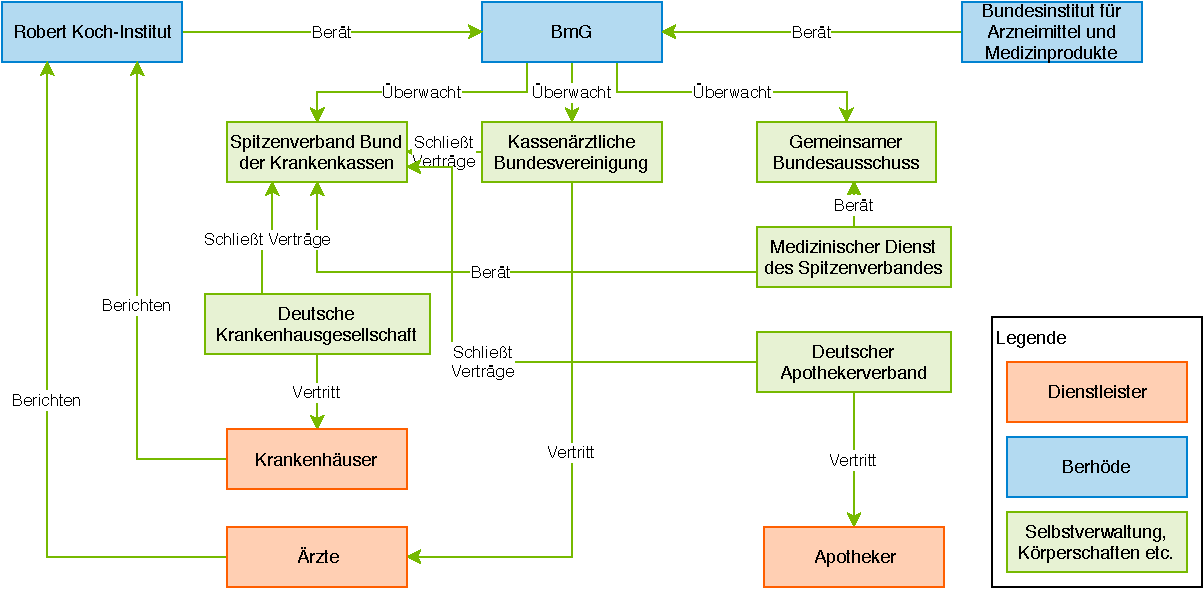
\includegraphics[height=5.5cm, right]{Bilder/GesundheitssystemAkteureBund.pdf}
        \caption{Einige Interaktionen auf Bundesebene. Eigene Abbildung.}
    \end{figure}
\end{frame}

\begin{frame}{Herausforderungen}
    \note{
        \begin{itemize}
            \item Steigende Anzahl an Ärzten
            \item Sinkende Zeit pro Patient
            \item Gründe: 
            \begin{itemize}
                \item Demographischer Wandel
                \item Bessere Behandelbarkeit trivialer Erkrankungen führt zu mehr chronischen und komplexen Erkrankungen
                \item<4> Zunehmende Pflegebedürftigkeit
                \item<4> Steigende Dokumentationspflichten
                \item<4> Steigende Komplexität der Diagnose/Behandlung
            \end{itemize}
        \end{itemize}
    }
    \begin{minipage}{.4\textwidth}
        \begin{figure}[h!]
            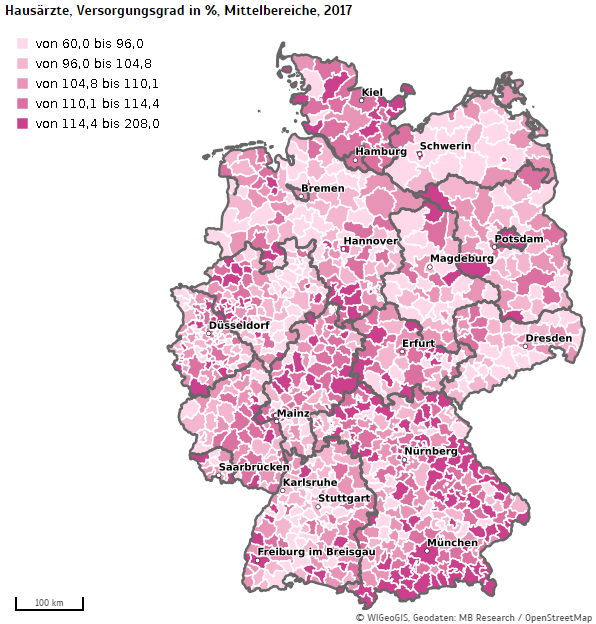
\includegraphics[height=5.5cm]{Bilder/HausarztVersorgung.png}
            \caption{Versorgung mit Hausärzten in 2018 \cite{HausarztVersorgung}}
        \end{figure}
    \end{minipage}
    \only<2->{
        \begin{textblock}{10}(6,0.5)
            \begin{figure}[h!]
                \frame{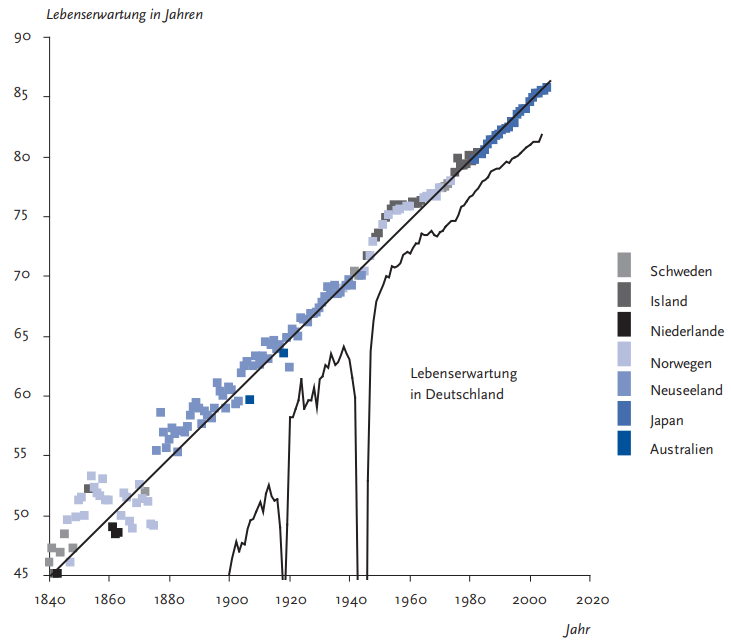
\includegraphics[width=6cm]{Bilder/Rekordlebenserwartungen.PNG}}
                \caption{Anstieg der Rekordlebenserwartung und der Lebenserwartung in Deutschland \cite{GesundheitKrankheitAlter}}
            \end{figure}
        \end{textblock}
    }
    \only<3->{
        \begin{textblock}{10}(6.7,6.7)
            \begin{figure}[h!]
                \frame{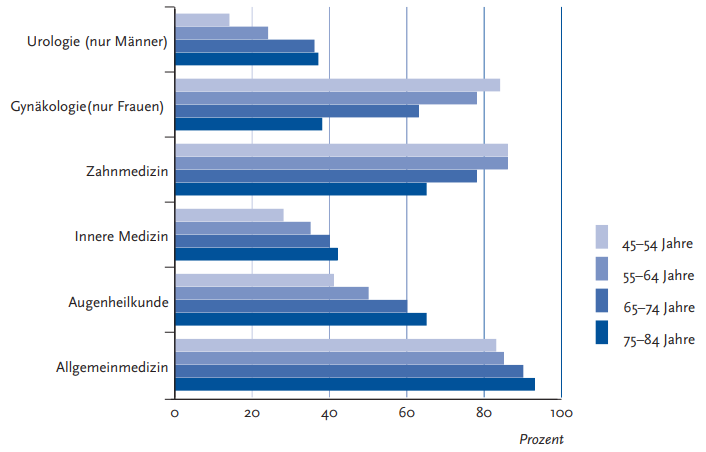
\includegraphics[width=6cm]{Bilder/InanspruchnahmeAerzte.png}}
                \caption{Inanspruchnahme von Ärzten (letzte 12 Monate) nach Alter und Arzt \cite{GesundheitKrankheitAlter}}
            \end{figure}
        \end{textblock}
    }
    \only<4->{
        \begin{textblock}{10}(2.8,3.8)
            \begin{figure}[h!]
                \frame{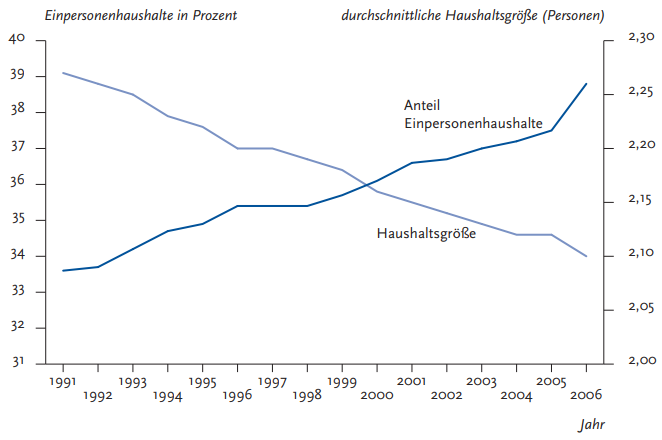
\includegraphics[width=6.5cm]{Bilder/Einpersonenhaushalte.png}}
                \caption{Entwicklung der Haushaltsgröße \cite{GesundheitKrankheitAlter}}
            \end{figure}
    \end{textblock}
    }
\end{frame}

\begin{frame}{IT-Unterstützung}
  \note{
  \begin{itemize}
      \item UC: Z.B. Blutdruck, Blutzucker, Sturzsensor, Lokationssensor (Wandern von Alzheimer-Patienten), Schweiß- und Herzfrequenzüberwachung zur Vorhersage epileptischer Anfälle etc.
      \item Benachrichtigung in Stufen, z.B. Angehörige, dann Pflegepersonal
      \item Erinnerung an Medikamente (Problem: Adhärenz!)
      \item Generell: Ortsunabhängige Pflege (zu Hause)
      \item Therapieunterstützung: Z.B. Kommunikation bei Depression, Gefühlstagebuch
      \item <2-> Automatische Übertragung von Geräten zu zentralen Datenbanken, automatische Vorauswertungen von Bilddaten
      \item<2-> Standardisierung - großes Problem in Medizintechnik
      \item<3-> Abgleich verschriebener Medikamente mit gelber oder roter Liste
      \item<5-> Automatische Benachrichtigung bei Ablauf von Blutkonserven, RFID-Kennzeichnung von OP-Besteck um Desinfektionszyklen einzuhalten etc.
  \end{itemize}}
  \begin{itemize}
      \item Ubquitous Computing: Sensorik und automatische Benachrichtigungen, insbesondere in der Pflege
      \item Telemedizin, Therapieunterstützung
      \item<2-> Verbesserung der Technikintegration
      \item<3-> Expertensysteme zur Behandlungsunterstützung
      \item<4-> Dokumentationsunterstützung
      \item<5-> Logistik
      \item<6-> Allgemein: Entlastung und Effizienzsteigerung, um bei gleichem Personal mehr Zeit für die Patienten zu haben
  \end{itemize}
\end{frame}

\begin{frame}{Aber warum Apps?}
    \begin{columns}
        \begin{column}{0.5\textwidth}
            \only<2->{
                \vspace{-0.6cm}
                \begin{figure}
                    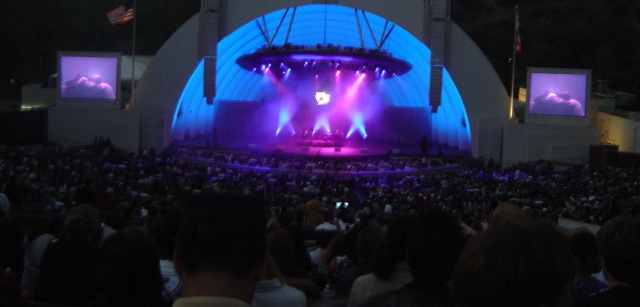
\includegraphics[width=0.75\textwidth]{Bilder/Concert2006.png}
                    \caption{Basement Jaxx, 2006 \cite{Concert2006}}
                \end{figure}
                \vspace{-1cm}
                \begin{figure}
                    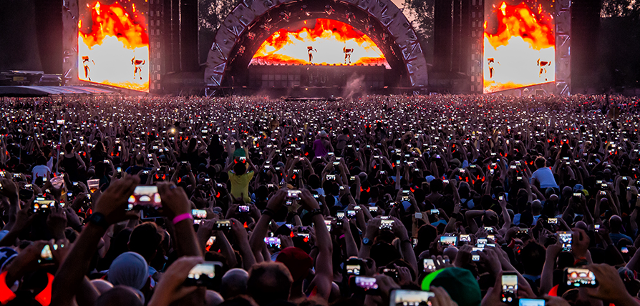
\includegraphics[width=0.75\textwidth]{Bilder/Concert2015.png}
                    \caption{AC/DC, 2015 \cite{Concert2015}}
                \end{figure}
            }
        \end{column}
        \begin{column}{0.5\textwidth}
            \begin{itemize}
                \item<3-> Durchdringung des Berufs- und Privatlebens mit digitalen Services
                \item<3-> Mentalität: Live erleben, digital teilen - Ungeduld
                \item<4-> Steigende Verfügbarkeit und Abhängigkeit von Handys
            \end{itemize}
        \end{column}
    \end{columns}
\end{frame}

\begin{frame}{App-Beispiel}
    ``Ich selbst habe eine App auf dem Handy, die mit 20 oder 30 Fragen Diagnosen genauer trifft als viele Ärzte, weil sie auf so viele Studien und Informationen zurückgreifen kann, wie es kein Arzt alleine kann.''\\
    Wer hat das über welche App gesagt?
    \only<2->{
        \\\vspace{0.5cm}Bundesgesundheitsminister Jens Spahn, 2018 \cite{SpahnApp} über ``Ada - Deine Gesundheitshelferin''.
    }
\end{frame}

\begin{frame}{ADA health companion}
    Google-Suche:
    \begin{itemize}
        \item \textit{A Look at Ada's AI-Powered Health Companion}: Ada's AI-powered health companion helps individuals understand and manage their health. In practice, Ada works much like a GP in your pocket. \cite{ADA1}
        \item<2-> \textit{Ada is an AI-powered doctor app and telemedicine service}: In my brief testing of the app, I plugged in the symptoms of a sore or red eye. After drilling through a quite extensive set of questions, many of which appeared to relate to the answers I’d previously given, the Ada app provided three possible conditions, and advised that they could be successfully treated at home. \cite{ADA2}
        \item<3-> \textit{Health companion app Ada Health raises EUR 40 million in first funding round} \cite{ADA3}
    \end{itemize}
\end{frame}

\begin{frame}{ADA health companion II}
    Gezielte Suche nach Studien zu Zuverlässigkeit:
    \begin{itemize}
        \item \textit{Doctors warn over diagnosis apps amid Ada launch}: Both the Australian Medical Association and Royal Australian College of GPs said they were concerned about the accuracy of the Ada system, and its potential to either falsely reassure people about their health or alarm them unnecessarily. \cite{ADA4}
        \item<2-> \textit{'Trust but verify' – five approaches to ensure safe medical apps}: We eagerly look forward to a time when medical apps might be relied upon to do much more complex tasks than simply calculate formulae or illustrate inhaler technique. [...] The potential for benefit remains vast and the degree of innovation is inspiring, but it turns out we are much earlier in the maturation phase of medical apps than many of us would have liked to believe. \cite{ADA5}
    \end{itemize}
\end{frame}

\begin{frame}{ADA health companion III}
    Fragwürdiger Umgang mit sensiblen Kundendaten:
    \begin{itemize}
        \item \textit{Ada nutzt Tracking- und Analyse-Dienstleister wie Amplitude, Adjust und Facebook}: Dabei werden Daten bereits übermittelt, bevor der Nutzer die AGB und Datenschutzerklärung gelesen und diesen zugestimmt hat. Dies steht im Widerspruch zur DSGVO, welche besagt, dass bei der Erhebung personenbezogener Daten die betroffene Person \textit{'zum Zeitpunkt der Erhebung dieser Daten'} informiert werden muss. \cite{ADA6}
        \item<2-> \textit{Übertragung von Daten in die USA}: Analysten von Heise Online habe herausgefunden, dass in Version 2.49.0 der App der Name der Krankenkasse von Nutzern an Facebook übermittelt wird. Darüber hinaus werden auch Symptombeschreibungen an Amplitude gesendet. (z.B. 'Herzrasen') \cite{ADA6}
    \end{itemize}
\end{frame}

\begin{frame}{Ökosystem}
    \begin{columns}
        \begin{column}{0.5\textwidth}
            \begin{figure}
                \centering
                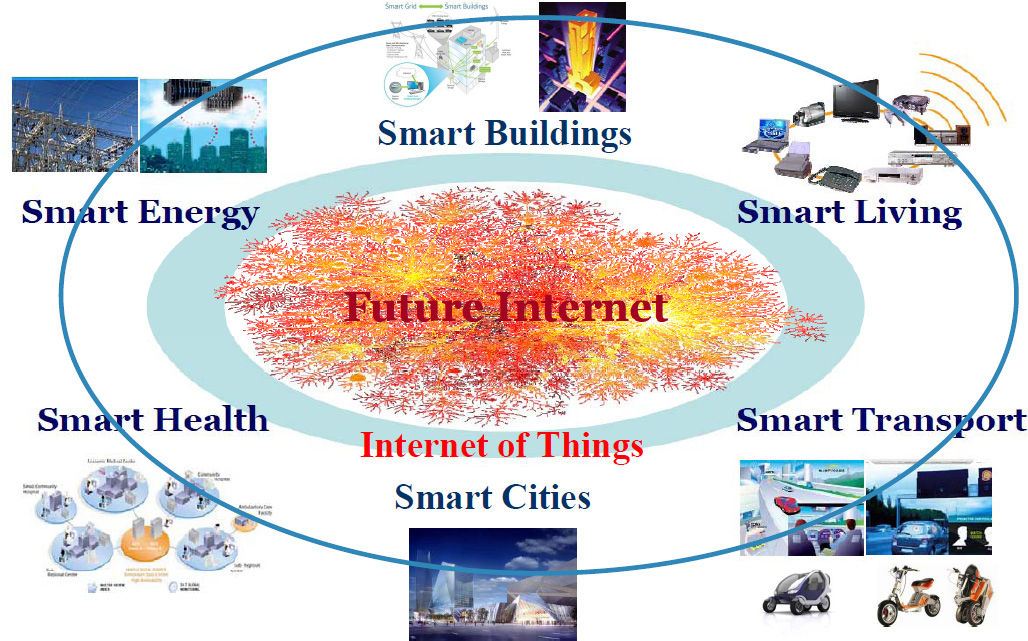
\includegraphics[width=\textwidth]{Bilder/Iot_apps.jpg}
                \caption{IoT, Smart Cities und Smart Health \cite{IoTapps}}
            \end{figure}
        \end{column}
        \begin{column}{0.5\textwidth}
            Gesundheits-Apps leben nicht isoliert.\\\vspace{0.5cm}
            \only<2->{
                ``The  maturation  and  adoption  of  computing  technologies have  dramatically  changed  the  face  of  healthcare. [...] In  the long  term,  integrating  technology  into  city-wide healthcare can reduce costs for the city and its citizens.'' \cite{Smart}
            }
        \end{column}
    \end{columns}
\end{frame}


\begin{frame}{Rahmenbedingungen}
    \note{
        Whiteboard-Aufgabe: Wann kann eine Gesundheits-App gefährlich sein? 
        \textbf{Zeit: Max. 5 Minuten}, wenn Fertig: Namensschild auf Bildschirm.
        \\KI: Großes Interesse, 
    }
    Kann von Apps eine Gefahr ausgehen?
    \only<2->{
        Einige Beispiele:
        \begin{itemize}
            \item Folgen von Fehlfunktionen, z.B. Einnahme falscher Medikamente
            \item<2-> Fehldiagnose, zu später Arztbesuch
            \item<3-> ``29 Prozent der Deutschen sehr oder ziemlich an einem Service interessiert, der den möglichen Einfluss der aktuellen Ernährungsweise auf die künftige Gesundheit ermittelt'' \cite{InteresseKI} - zu hohes Vertrauen?
            \item<3-> Falsche Haltung/Intensität bei Übungen
            \item<4-> Abfluss persönlicher Daten: ``Gesundheits-Apps halten die datenschutzrechtlichen Anforderungen häufig nicht ein'' \cite{CHARISMABMG}
            \item<5-> Verlust von Körpergefühl, Verstärkung von Krankheitsängsten (Cyberchondrie)
        \end{itemize}
    }
    \only<6->{...also müsste es irgendeine Regelung geben?}
    \only<7->{ $\rightarrow$ Medizinproduktegesetz.}
\end{frame}

\begin{frame}{Gefahren von medizinischen Apps}
    Ihre Bedenken beim Einsatz von medizinischen Apps zusammengefasst:
    \begin{itemize}
        \item Zu komplexe Fragestellung, um aufgrund selbst aufgenommener Daten eine sichere Diagnose zu erstellen, dadurch Fehldiagnosen
        \item Fehldiagnosen durch fehlenden Sachverstand der Entwickler
        \item Fehlbenutzung, die z.B. zu Fehldiagnosen oder Fehlhaltungen bei Physitherapie-Übungen führt
        \item Klau von Daten oder Verkauf von Daten an Versicherungen, die z.B. Prämienerhöhungen daraus berechnen
    \end{itemize}    
\end{frame}

\begin{frame}{Teambildung: Vorstellung}
    \note{
        Um das Ganze ein wenig aufzulockern...
        \begin{itemize}
            \item Ziel: Entwicklung einer App im 5er-Team
            \item Manche haben mehr, manche weniger technischen Background
            \item Studierende aus IMI anwesend, wichtige Kompetenz!
            \item Informationen, um ausgewogene Teams zu erstellen
        \end{itemize}
        Zeit: 10 Minuten. \textbf{Wenn fertig, Namensschild auf Bildschirm!}
        \\
        Man glaubt gar nicht, wie häufig man sich kurz vorstellen muss - guten Eindruck machen ist wichtig, also üben!
        \\
        \textbf{Aufgabe für alle}: Notizen machen! Interessante Details (``Kann was was ich nicht kann'', ``Gute Idee'', ...) - mit wem wollen Sie zusammenarbeiten, wen ansprechen? Wen würden Sie einstellen, wenn Sie gerade ihr Startup gründen?
    }
    \only<2->{
        Kurzprofil:
        \begin{itemize}
            \item Name
            \item Bisherige Erfahrung (Sprachen, Projekte etc.) in:
            \begin{itemize}
                \item Programmierung
                \item App-Entwicklung
                \item (UI-)Design
            \end{itemize}
            \item Relevante Interessen, idealerweise mit erster App-Idee
        \end{itemize}
    }
    \only<3->{Vorstellung: 2 Minuten + Profilbogen}
\end{frame}

\begin{frame}{Ergebnis der Gruppenbildung}
    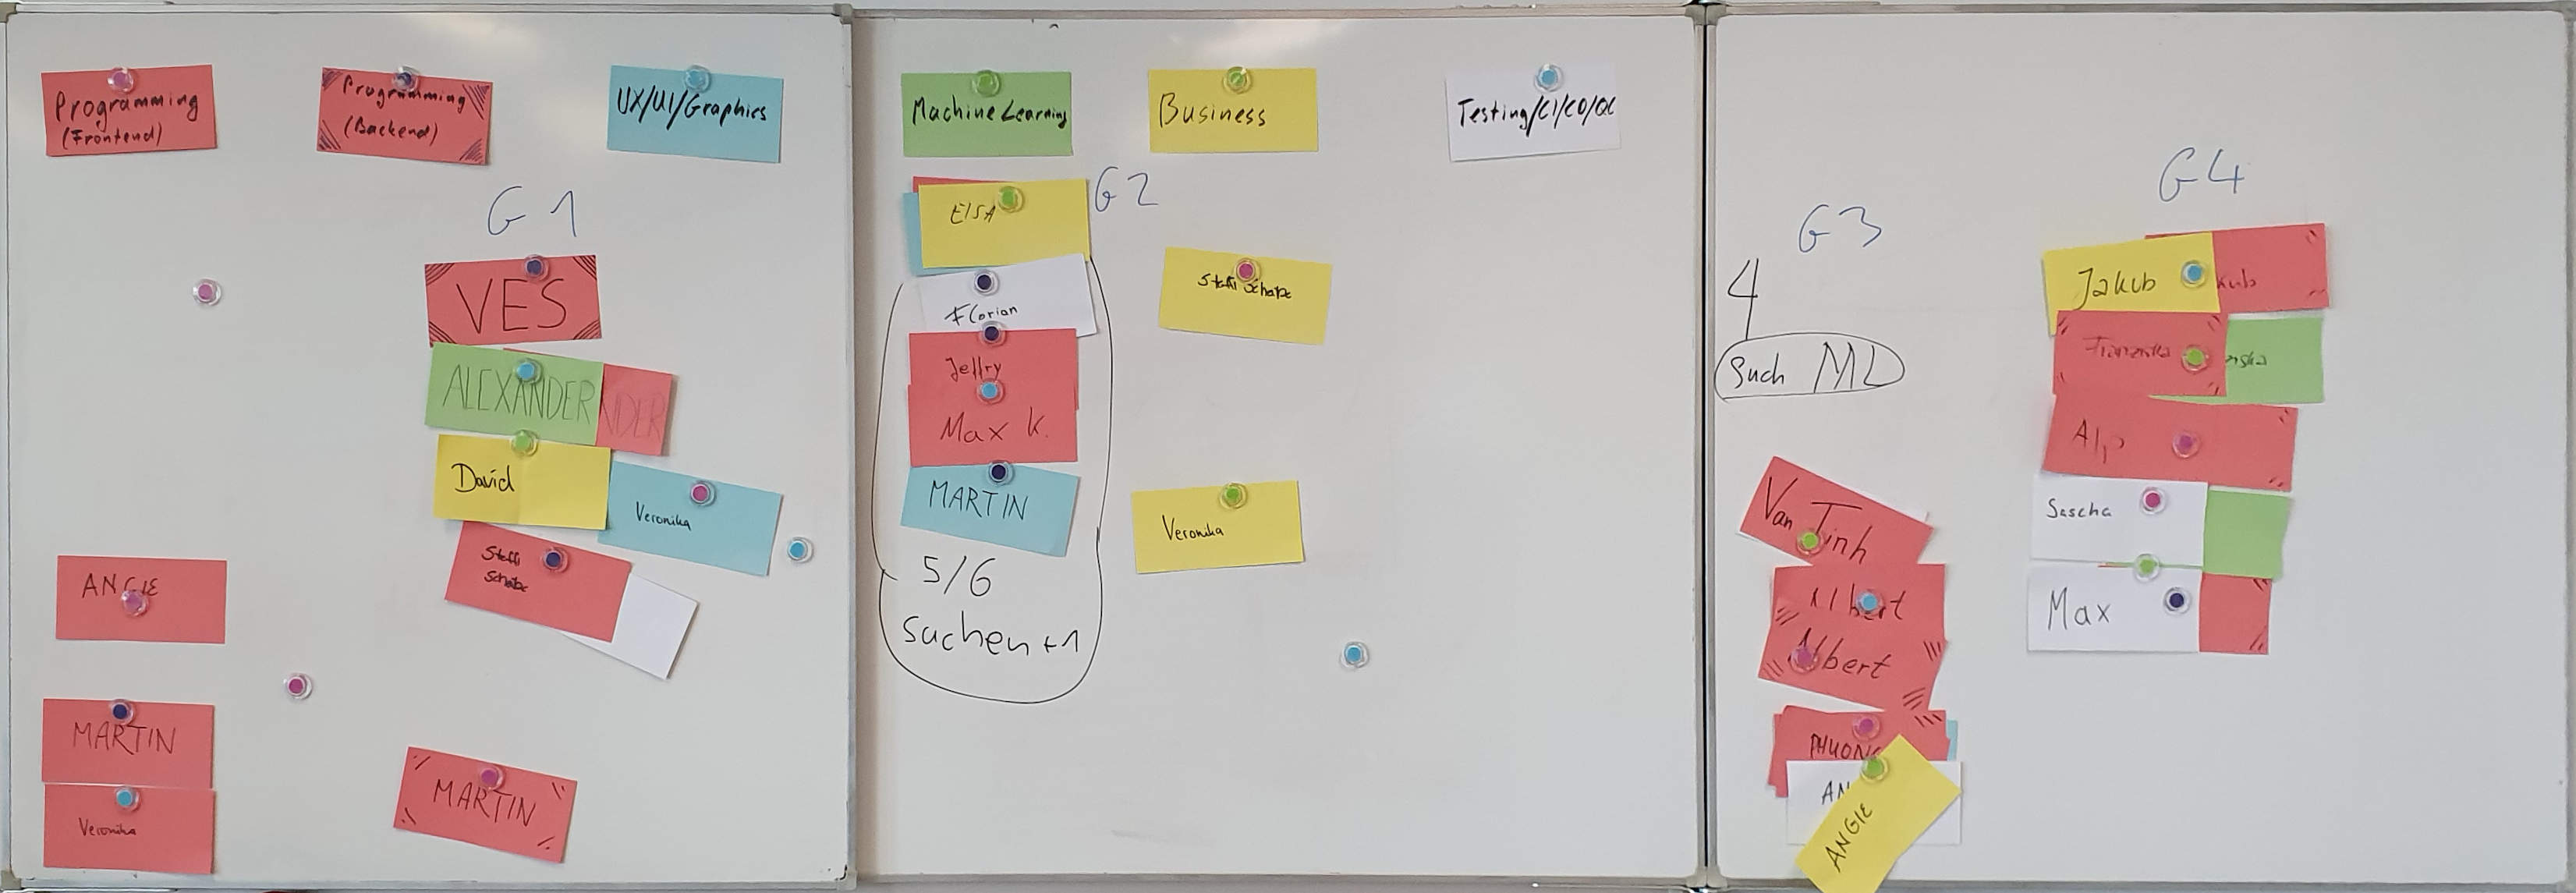
\includegraphics[width=\textwidth]{Bilder/groups.jpg}
\end{frame}

\begin{frame}{Medizinprodukte}
    \note{
        Alles, was kein Medikament ist und bei der
        \begin{itemize}
            \item Erkennung
            \item Verhütung
            \item Überwachung
            \item Behandlung
            \item Linderung
            \item Kompensierung
        \end{itemize}
        von Krankheiten, Verletzungen oder Behinderungen oder bei der Empfängnisregelung hilft (und durch Medikamente unterstützt werden kann). 
    }
    \footnotesize{
        Medizinprodukte sind alle einzeln oder miteinander verbunden verwendeten Instrumente, Apparate, Vorrichtungen, Software, Stoffe und Zubereitungen aus Stoffen oder andere Gegenstände einschließlich der vom Hersteller speziell zur Anwendung für diagnostische oder therapeutische Zwecke bestimmten und für ein einwandfreies Funktionieren des Medizinproduktes eingesetzten Software, die vom Hersteller zur Anwendung für Menschen mittels ihrer Funktionen zum Zwecke
        \begin{itemize}
            \item der Erkennung, Verhütung, Überwachung, Behandlung oder Linderung von Krankheiten,
            \item der Erkennung, Überwachung, Behandlung, Linderung oder Kompensierung von Verletzungen oder Behinderungen,
            \item der Untersuchung, der Ersetzung oder der Veränderung des anatomischen Aufbaus oder eines physiologischen Vorgangs oder
            \item der Empfängnisregelung
        \end{itemize}
        zu dienen bestimmt sind und deren bestimmungsgemäße Hauptwirkung im oder am menschlichen Körper weder durch pharmakologisch oder immunologisch wirkende Mittel noch durch Metabolismus erreicht wird, deren Wirkungsweise aber durch solche Mittel unterstützt werden kann.
    }
\end{frame}

\begin{frame}{Medizinproduktegesetz}
    \note{
        Ziel: Keine große Expertise in MPG aufbauen, das wäre eigene VL. Gefühl für die Komplexität bekommen! (heißt aber nicht ``nicht klausurrelevant''!)\\
        Wichtig zu bedenken: Ursprünglich und hauptsächlich Gedanke an Prothesen, Bandagen etc., aber auch anwendbar auf Gesundheits-Apps!
        \\
        \textbf{Risikoklasse}: Apps meist Klasse \textbf{I}, außer z.B. Verhütung/STD-Verhinderung Klasse \textbf{IIb}, Diagnose oder Kontrolle von Vitalfunktionen \textbf{IIa oder IIb}
        \\
        \textbf{ZLG}: Zentralstelle der Länder für Gesundheitsschutz bei Arzneimitteln und Medizinprodukten
    }
    Das MPG regelt den Umgang mit Medizinprodukten. Unter Anderem:
    \begin{itemize}
        \item Wann das Inverkehrbringen verboten ist
        \only<1>{
            \begin{itemize}
                \item Wenn Verdacht auf Gefährdung besteht
                \item Wenn sie Leistung versprechen, die sie nicht erbringen
                \item Sicherer Erfolg/Schadensfreiheit versprochen wird aber nicht garantiert werden kann
            \end{itemize}
        }
        \item<2-> Vorgehen beim Inverkehrbringen
        \only<2>{
            \begin{itemize}
                \item Verantwortlich: Hersteller, \textbf{Einführer} oder Bevollmächtigter
                \item Einordnung in Risikoklasse (93/42/EWG)
                \item CE-Kennzeichen notwendig (außer Klasse I durch ZLG benannte Benannte Stelle)
                \item Verständliche Anleitung in Deutscher Sprache
            \end{itemize}
        }
        \item<3-> Details zur klinischen Bewertung und Leistungsbewertung
        \only<3>{
            \begin{itemize}
                \item Klinische Bewertung anhand klinischer Daten notwendig, falls nicht andere Daten ausreichend sind (begründete Ausnahmefälle sowie in-vitro-Diagnostika)
                \item Klinische Prüfung nur mit Genehmigung der Ethikkommission, Patienteneinwilligung etc.
            \end{itemize}
        }
        \item<4-> Überwachung
        \only<4>{
            \begin{itemize}
                \item Meldepflicht für Verantwortliche
                \item Rechte der Behörden zur Überprüfung (Betretung und Besichtigung von Geschäftsräumen, Prüfung von Produkten und Unterlagen etc.)
                \item Anordnung zur Schließung des Betriebs bei Gefahr für öffentliche Gesundheit
            \end{itemize}
        }
        \item<5-> Strafen, z.B.
        \only<5>{
            \begin{itemize}
                \item Unerlaubtes Inverkehrbringen oder Betreiben: Bis 3 Jahre
                \item Unerlaubtes Anbingen von CE-Kennzeichen: Bis 1 Jahr
                \item Unerlaubtes Anwenden eines in-vitro-Diagnostikums: Bis 30'000 Euro
                \item Eine Überwachungsmaßnahme nicht zulassen: Bis 30'000 Euro
            \end{itemize}
        }
    \end{itemize}
    \only<6->{Aber: Nicht jede Gesundheitsapp ist ein Medizinprodukt! Abgrenzung: Apps für reine Sportzwecke, Fitness, Wellness oder Ernährung. Siehe auch BfArM-Orientierungshilfe \cite{BfArMOrientierungshilfe}.}
    \only<7>{\\\textbf{Wichtig}: Das sind nur die Regeln in Deutschland. Andere Länder, andere Regeln, andere Strafen!}
\end{frame}

\stepcounter{slidesection}
\setbeamertemplate{background}[bgfirst]
\setbeamertemplate{footline}[first]
\subtitle{\theslidesection: Entwicklungsaufgabe}
\titlegraphic{Bilder/logo3.jpg}
\begin{frame}[noframenumbering]
    \titlepage
    \begin{textblock}{10}(4.75,15)
        \cite{logo3}
    \end{textblock}
\end{frame}
\setbeamertemplate{footline}[presentationbody] 
\setbeamertemplate{background}[bgbody]

\begin{frame}{Startup-Gründung}
    \note{
        Idee: Vielleicht noch nicht, machen wir aber im Ideenfindungs-Workshop!
    }
    Sie haben:
    \begin{itemize}
        \item Team und Willen, ein Startup zu gründen
        \item Eine Idee für eine Gesundheits-App
        \item Kontakte zu Investoren
    \end{itemize}
    \only<2->{
        Sie brauchen:
        \begin{itemize}
            \item Einen Business-Plan
            \item Ein Proof-of-Concept
        \end{itemize}
    }
    \only<3->{...und das in 4 Monaten! Was nun?}
\end{frame}

\begin{frame}{Zielgruppe finden}
    Wo gibt es:
    \begin{itemize}
        \item Viele potentielle Anwender
        \item Großen Lösungsbedarf
        \item Großes Verbesserungspotential
        \item Allgemein: Hohes Marktpotential
    \end{itemize}
\end{frame}

\begin{frame}{Zielgruppe finden}
    \begin{figure}
        \centering
        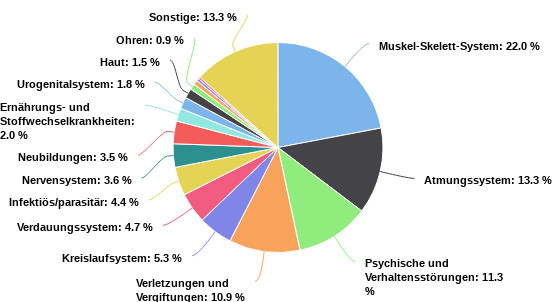
\includegraphics[width=0.7\textwidth]{Bilder/Krankheitstage.jpg}
        \caption{Anteil der Krankheitstage (Gesamt 510 Millionen) AOK-Versicherter nach Diagnose. Eigene Abbildung, Daten der GBE Bund \cite{GBEKrankheitstage}}
    \end{figure}
\end{frame}

\begin{frame}{Zielgruppe finden}
    \note{
        \begin{itemize}
            \item Alkohol: $10\%$ der Arbeitnehmer risikant
            \item Spiele: $6.5\%$ der Arbeitnehmer risikant
            \item Neubildungen: Nur $3.5\%$ Fehltage, aber teures und großes Risiko für z.B. Bauarbeiter. UV-Vorhersage-Apps
        \end{itemize}
        
    }
    \begin{itemize}
        \item Muskel-Skelett-System: Laut Ärzteblatt hat jeder 3. Erwachsene Rückenbeschwerden
        \item Depression: Laut WHO 4.6 Millionen Deutsche mit Depression
        \item Suchtprobleme (Alkohol, Spiele, Rauchen): Laut DAK-Gesundheitsreport 2019 über $10\%$
        \item Wohlstandskrankheiten, demografischer Wandel
    \end{itemize}
\end{frame}

\begin{frame}{Lösungsidee erarbeiten}
    \note{
        Was hilft? Wie kann man es mit Technologie unterstützen? Viele Ideen hatten schon andere Leute.
        \\Kamera: Nicht unterschätzen, z.B. LFA-Analyse
        \\Mikrofon: Z.B. Schnarchgeräusche
        \\Sensoren: Nachteile extern:
        \begin{itemize}
            \item Müssen rumgetragen werden
            \item Probleme mit Konnektivität, kaum Standards
            \item Veraltern schnell
            \item Teuer
        \end{itemize}
    }
    \noindent Erstens: Literaturrecherche!
    \only<2->{\\\noindent Großer Mehrwert des Handys: Sensorik}
    \begin{columns}
        \begin{column}{0.5\textwidth}
            \only<3->{
                Intern:
                \begin{itemize}
                    \item Accelerometer
                    \item Gyroskop
                    \item Magnetometer
                    \item GPS
                    \item Näherungsschalter
                    \item Barometer
                    \item Umgebungslichtsensor
                    \item Kamera, Mikrofon
                \end{itemize}
            }
        \end{column}
        \begin{column}{0.5\textwidth}
            \only<4->{
                Extern:
                \begin{itemize}
                    \item Herzfrequenz
                    \item Temperatur
                    \item Blutdruck
                    \item Oximeter
                    \item EMG
                    \item Glucometer
                    \item ...
                \end{itemize}
            }
        \end{column}
    \end{columns}
\end{frame}

\begin{frame}{Beispiel für Sensor-Integratoin}
	\href{https://www.kenkou.de/}{Kenkou} - App zur Stressbewältigung. Medizinprodukt nach MPG: Empfiehlt Übungen je nach Stresslevel. 
	\begin{itemize}
		\item Messung des Blutflusses durch Helligkeitsveränderungen der Blutgefäße in der Fingerkuppe
		\item Berechnung der Herzratenvariabilität
		\item<2-> Verwendung von Blitzlicht+Kamera als Messgerät
		\item<3-> Training auf großen Datenmengen, um Aussagen zu Stresslevel zu erlauben
		\item<4-> Anreicherung mit Nutzer-Angaben zur Erhöhung der Zuverlässigkeit
		\item<5-> ...Datenschutz?
	\end{itemize}
\end{frame}

\begin{frame}{Wann wird eine App erfolgreich?}
    \note{
        Idee und Lösungsansatz da. Wie bringt man es unter die Anwender?
        \begin{itemize}
            \item Nutzerfreundlichkeit: Auch Performance, Einfachheit
            \item Leistungserbringer: Networking, Ärzte-Kongresse
        \end{itemize}
    }
    ``Unsere App würde das Leben der Leute viel besser machen, aber keiner nutzt sie''...
    \begin{itemize}
        \item<2-> Nutzerfreundlichkeit
        \only<2>{
            \begin{itemize}
                \item Einfach zugängliche Information, Visualisierung
                \item Orts- und Geräteunabhängige Nutzung
                \item Kein ``Nerven'', keine/nicht störende Werbung
                \item Klare Information zu Datenschutz
                \item Individualisierbarkeit
            \end{itemize}
        }
        \item<3-> Problemlösung
        \only<3>{
            \begin{itemize}
                \item Nachweis des Therapie-Nutzens
                \item Zuverlässigkeit der Daten/Berechnungen
                \item Integration medizinischer Expertise
            \end{itemize}
        }
        \item<4-> Spaßfaktor
        \only<4>{
            \begin{itemize}
                \item Fortschrittsgefühl
                \item Belohnung
                \item Gamification?
            \end{itemize}
        }
    \end{itemize}
    \only<5->{
        Und idealerweise ein Geschäftsmodell...
        \begin{itemize}
            \item<6-> Leistungserbringer \only<7>{``ONCOassist generates revenue by working both independently and in collaboration with the pharmaceutical industry to integrate tools and content which helps improve patient care'' \cite{ONCOassist}}
            \item<8-> Kostenerstattung \only<9>{``Die Techniker Krankenkasse übernimmt bundesweit für ihre Versicherten die Kosten für ein 6-monatiges Training mit der neolino-App'' \cite{neolino}}
            \item<10-> Gesellschaft, Politik, aktuelle Technik-Trends \only<11>{``Bundesregierung stärkt die Förderung Künstlicher Intelligenz mit zusätzlichen 500 Millionen Euro'' \cite{KIfoerderung}}
        \end{itemize}
    }
\end{frame}

\begin{frame}{Beispiel für erfolgreiche App}
    \note{
        \begin{itemize}
            \item Modell: Freie App, Geräteintegration etc. als Abo. Erstattbarkeit und Pakete durch Krankenkassen
            \item Erfolgskriterien:
            \begin{itemize}
                \item Klarer Bedarf!
                \item Qualität (``Eat your own dogfood'')
                \item Einbindung der Community
            \end{itemize}
            \item Mitfinanzierung durch staatliche Start-up-Fonds
            \item 5 Jahre bis zum finanziellen Erfolg: ``Wir haben unser privates Geld, Zeit, in manchen Fällen sogar den Wohnort geopfert''
        \end{itemize}
    }
    \begin{columns}
        \begin{column}{0.6\textwidth}
            \vspace{-0.7cm}
            \begin{figure}
                \begin{minipage}{0.33\textwidth}
                    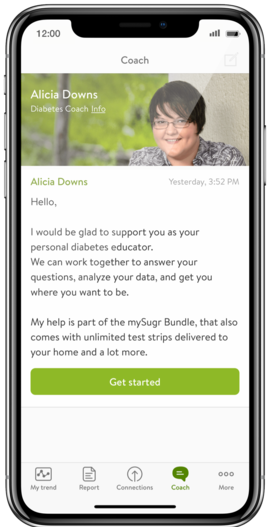
\includegraphics[width=\textwidth]{Bilder/mysugr1.png}
                \end{minipage}%
                \begin{minipage}{0.33\textwidth}
                    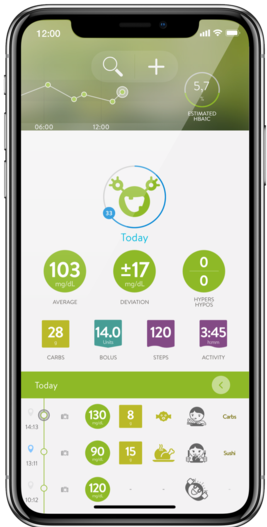
\includegraphics[width=\textwidth]{Bilder/mysugr2.png}
                \end{minipage}%
                \begin{minipage}{0.33\textwidth}
                    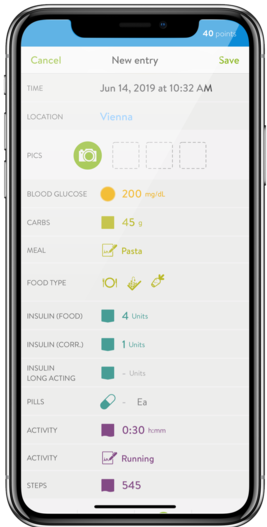
\includegraphics[width=\textwidth]{Bilder/mysugr3.png}
                \end{minipage}
                \vspace{0.1cm}
                \caption{Screenshots der App mySugr \cite{mysugr}}
            \end{figure}    
        \end{column}
        \begin{column}{0.4\textwidth}
            \noindent mySugr: App für Diabetiker
            \begin{itemize}
                \item[2011] Ein Diabetiker will sein Diabetik-Tagebuch digital führen, hat das Handy immer dabei
                \item[2012] Unternehmensgründung
                \item<2->[2017] Kauf durch Roche. ``Über den Kaufpreis [...] herrscht Stillschweigen, von einer dreistelligen Millionensumme darf ausgegangen werden.'' \cite{mysugrverkauf}
            \end{itemize}
        \end{column}
    \end{columns}
    \begin{textblock}{15}(12.5,1)
        
\includegraphics[width=3cm]{Bilder/mysugrlogo.png}
    \end{textblock}
\end{frame}


\stepcounter{slidesection}
\setbeamertemplate{background}[bgfirst]
\setbeamertemplate{footline}[first]
\subtitle{\theslidesection: Technische Grundlagen}
\titlegraphic{Bilder/logo2.png}
\begin{frame}[noframenumbering]
    \titlepage
    \begin{textblock}{10}(4.75,15)
        \cite{ProgrammingLogo}
    \end{textblock}
\end{frame}
\setbeamertemplate{footline}[presentationbody] 
\setbeamertemplate{background}[bgbody]


\begin{frame}{Sourcecodeverwaltung}
    \note{
        Bevor wir anfangen, Code zu schreiben, müssen wir uns Gedanken darüber machen, wie wir das tun...
        \begin{itemize}
            \item Perforce
            \begin{itemize}
                \item Einsatz in großen Unternehmen (größtes Repo bei Google, 18/20 top-Spieleherstellern, Netflix etc.)
                \item Ändert darunterliegende Technologie nach Bedarf (aktuell git.kompatibel, aber erste Version 10 Jahre vor git)
            \end{itemize}
            \item Subversion: Tracking von Verschieben, Umbenennen etc.
            \item git: Durch Kommerzialisierung von BitKeeper
            \item mercurial: Gleiches Ziel wie git (Linux-Kernel), heutzutagez.B. bei Facebook und Mozilla im Einsatz
            \item Einer der großen heiligen Kriege: git vs. mercurial
            \item Derzeit primär im Einsatz: SVN, Perforce, TFS (zentral), git, mercurial (dezentral)
        \end{itemize}
    }
    \begin{itemize}
        \item Ursprüngliche Herangehensweise: Datei\_final\_final\_realfinal\_12.java...
        \item<2-> 1972: Bell labs, SCCS (source code control system, single user, nur Textdateien)
        \item<3-> 1986: CVS (concurrent version system, zentral, dateibasiert)
        \item<4-> 1995: Helix core (Perforce)
        \item<5-> 2000: SVN (subversion, zentral, verzeichnisbasiert)
        \item<6-> 2004: TFS (team foundation server, Microsoft, zentral/git, verzeichnisbasiert mit bug tracker etc.)
        \item<7-> 2005: git (Linus Torvalds, dezentral, verzeichnisbasiert)
        \item<8-> 2005: mercurial (dezentral, verzeichnisbasiert)
    \end{itemize}
\end{frame}

\begin{frame}{Sourcecodeverwaltung (git)}
    \note{Abgabe von Übungsaufgaben nur als Release-Link in git-Repository}    
    \begin{minipage}{.4\textwidth}
        \begin{figure}[h!]
            \frame{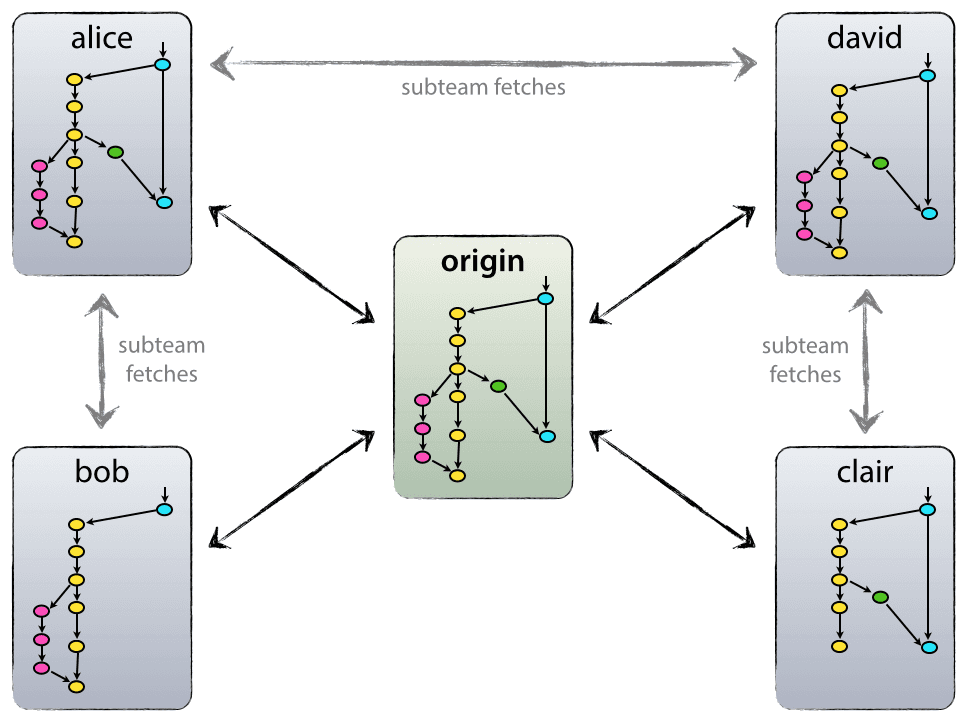
\includegraphics[height=5.5cm]{Bilder/gitbranching2.png}}
            \caption{Teamarbeit mit mehreren remotes \cite{gitbranching}}
        \end{figure}
    \end{minipage}
    \only<2->{
        \begin{textblock}{6}(10,0.2)
            \begin{figure}[h!]
                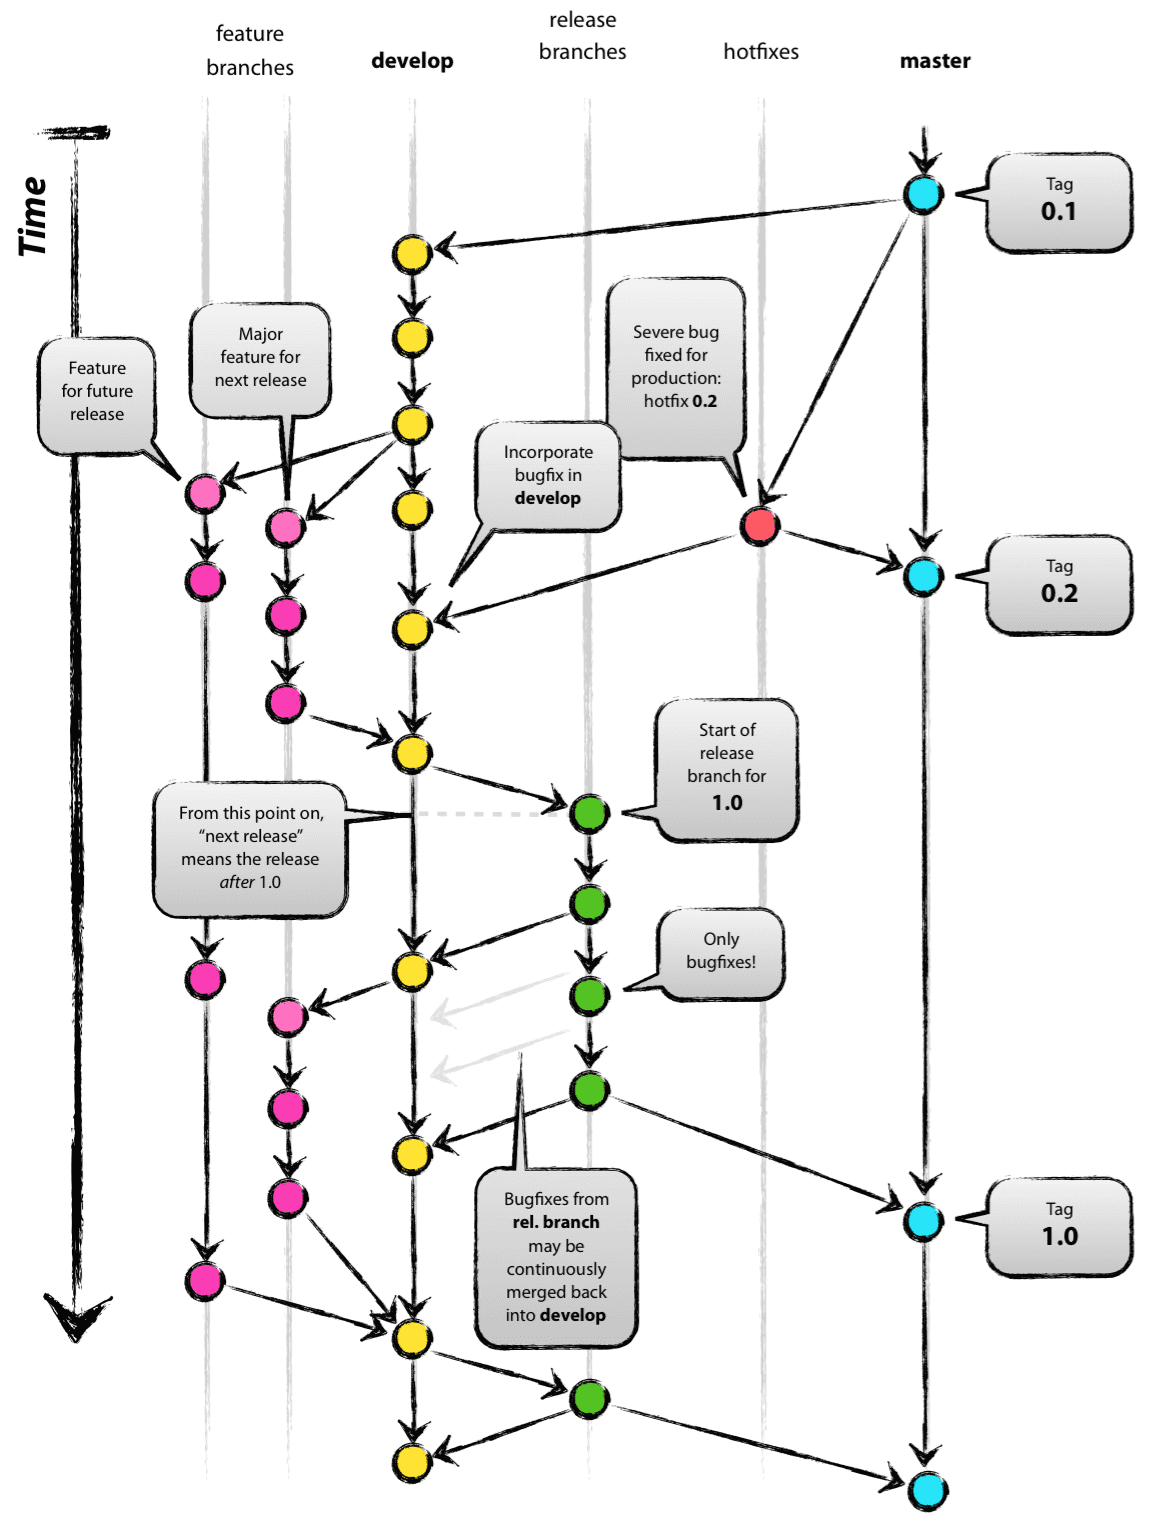
\includegraphics[height=7.3cm]{Bilder/gitbranching.png}
                \caption{Komplexe branching-Strategie \cite{gitbranching}}
            \end{figure}
        \end{textblock}
    }
\end{frame}

\begin{frame}{Flutter}
    \note{
        \only<1-2>{
            Wichtig: Keine Werbung für Flutter, zeigt Herangehensweise an neues Projekt (selber keine Erfahrung mit Flutter)
            Beispiele:\\Java super für portable, performante Applikationen, aber mies für Prototyping\\Python super für Prototyping, aber schlecht für Stabilität\\PHP Totalausfall bei Wartbarkeit+Sicherheit, aber toll für schnelle kleine Webapp\\Wünsche JavaScript schnellen und schmerzhaften Tod, setze es trotzdem für interaktive Visualisierungen ein\\etc... \\Fazit: Keine silver bullet, man muss viele Stärken und Schwächen kennen, und z.T. Programmierkonzepte zwischen Sprachen übertragbar. Flexibilität ist wichtig!
        }
        \only<3->{
            Mini-Whiteboard: Was ist wichtig bei der Entscheidung für eine Sprache für ein Projekt?
            \textbf{Zeit: 5 Minuten}
            \begin{itemize}
                \item Entwickler: Einer? Mehrere? Community oder Spaltungen? Aktivität der Entwicklung? (wikipedia)
                \item Anzahl an reifen Projekten in Sprache (flutter.dev)
                \item Bekannte Schwachstellen und Reaktionen (exploit-db.com, cve.mitre.org etc), konkretes Beispiel: www.cvedetails.com, Oracle (Page 10), Java, Metasploit modules, CVE-2012-4681 Java 7 Applet Remote Code Execution. Google: Page 12. Dart: Dart TCP
                \item Geeignetheit der Features für Problem (bsp. R, shell, PHP)
                \item Verfügbarkeit von relevanten Bibliotheken (pub.dev, chart, flchart)
                \item Verfügbarkeit aktueller Entwicklungstools
                \item Lizenz: Vorhanden? Falls ja, Bedingungen, bsp. GPL vs. LGPL. BSD: Redist license!
            \end{itemize}
        }
    }
    Wichtig in Programmierung: Weniger eine konkrete Sprache, mehr breites Wissen und Verständnis von Konzepten. Also: Richtige Programmiersprache für das Problem wählen! \only<2->{Aber: Was heißt ``richtig?''}\only<4->{\textbf{ Und ist Flutter ``richtig''?}}
    \only<3->{
        \begin{itemize}
            \item[\only<4>{\textbullet}\only<5->{\checkmark}] Aktive Entwicklung
            \item[\only<4-5>{\textbullet}\only<6->{\checkmark}] Starke Aktuere in der Community
            \item[\only<4-6>{\textbullet}\only<7->{\checkmark}] Vorhandensein reifer Produkte
            \item[\only<4-7>{\textbullet}\only<8->{\checkmark}] Sicherheit
            \item[\only<4-8>{\textbullet}\only<9->{\checkmark}] Relevante Bibliotheken und Entwicklungstools
            \item[\only<4-9>{\textbullet}\only<10->{\checkmark}] Bekannte und nutzbare Lizenz
            \item[\only<4-10>{\textbullet}\only<11->{?}] Ausreichende ROI bei fehlenden Vorkenntnissen
        \end{itemize}
    }
\end{frame}

